\chapter{Work, Power, and the Work-Energy Theorem}
\label{ch:work_energy}

\begin{chapterintro}
\textbf{Chapter Objectives:} In this chapter, we bridge Newton's differential equations of motion and scalar conservation laws. You will learn to formulate work rigorously as a curvilinear line integral along a trajectory; define instantaneous power; derive the Work-Energy (Kinetic Energy) theorem from first principles in both inertial and non-inertial frames; and apply scalar energy techniques to solve constrained mechanical systems including the vertical loop-the-loop and spherical dome detachment.
\end{chapterintro}

\section{Work as a Curvilinear Line Integral}

Newton's second law $\vec{F} = m\,\dd\vec{v}/\dd t$ provides a vector relationship linking force directly to acceleration. However, integrating this vector differential equation along arbitrary spatial paths is often analytically intractable. By projecting Newton's law onto the instantaneous direction of motion, we obtain a scalar formulation of fundamental generality: the concept of \textbf{mechanical work}.

\begin{definitionbox}{Elementary Mechanical Work}
Let a material point $M$ move under the action of a force $\vec{F}$ through an infinitesimal displacement $\dd\vec{r}$. The \textbf{elementary mechanical work} $\delta W$ performed by $\vec{F}$ is defined as the scalar product:
\begin{equation}
\delta W \eqdef \vec{F} \cdot \dd\vec{r}.
\end{equation}
In the SI system, work is measured in \textbf{joules} ($\mathrm{J}$), where $1\ \mathrm{J} = 1\ \mathrm{N\cdot m} = 1\ \mathrm{kg\cdot m^2\cdot s^{-2}}$.
\end{definitionbox}

The symbol $\delta W$ (rather than $\dd W$) is deliberately employed to emphasize that work is an \emph{inexact differential}: work represents a quantity of energy transferred along a specific trajectory, not the change in an intrinsic state property of the particle.

\begin{figure}[htbp]
\centering
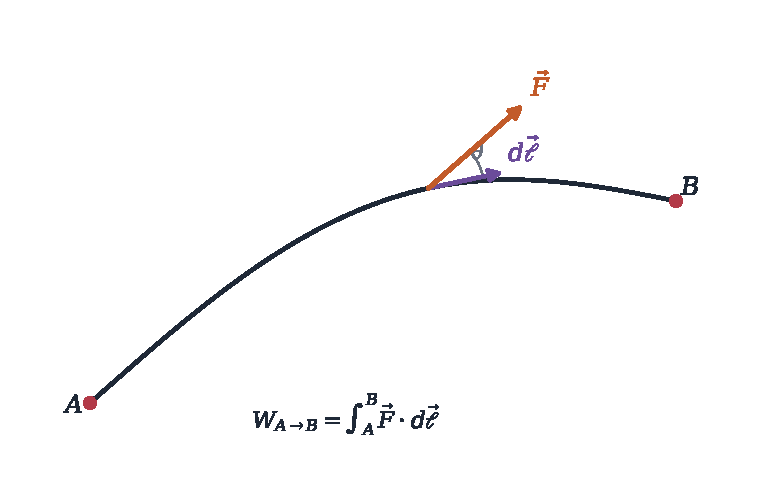
\includegraphics[width=0.74\textwidth]{figures/18_work_path.pdf}
\caption{Curvilinear trajectory $\mathcal{C}$ between states $A$ and $B$. The elementary work $\delta W = \vec{F}\cdot\dd\vec{r} = F_t\,\dd s$ represents the projection of the instantaneous force along the tangential unit vector $\utt$ multiplied by the arc length element $\dd s$.}
\label{fig:work_path}
\end{figure}

In different coordinate systems, the elementary work assumes distinctive explicit forms:
\begin{itemize}[leftmargin=1.5em,itemsep=4pt]
  \item \textbf{Cartesian coordinates:} With $\vec{F} = F_x\,\ihat + F_y\,\jhat + F_z\,\khat$ and $\dd\vec{r} = \dd x\,\ihat + \dd y\,\jhat + \dd z\,\khat$:
  \begin{equation}
  \delta W = F_x\,\dd x + F_y\,\dd y + F_z\,\dd z.
  \end{equation}
  \item \textbf{Frenet-Serret intrinsic coordinates:} Decomposing $\vec{F} = F_t\,\utt + F_n\,\un + F_b\,\ub$ and noting that $\dd\vec{r} = \utt\,\dd s$:
  \begin{equation}
  \delta W = (F_t\,\utt + F_n\,\un + F_b\,\ub) \cdot \utt\,\dd s = F_t\,\dd s.
  \end{equation}
  \emph{Key physical insight:} Normal and binormal forces ($\vec{F}_\perp = F_n\un + F_b\ub$) perform strictly zero mechanical work at every instant because they are perpendicular to the velocity vector $\vec{v} = \dot{s}\utt$.
  \item \textbf{Plane polar coordinates:} With $\vec{F} = F_r\,\ur + F_\theta\,\ut$ and $\dd\vec{r} = \dd r\,\ur + r\,\dd\theta\,\ut$:
  \begin{equation}
  \delta W = F_r\,\dd r + F_\theta\,r\,\dd\theta.
  \end{equation}
\end{itemize}

\begin{definitionbox}{Total Work Along a Finite Trajectory}
The total work performed by a force field $\vec{F}$ as the particle moves along a prescribed continuous path $\mathcal{C}$ from initial point $A$ to final point $B$ is the curvilinear line integral:
\begin{equation}
W_{A \to B} \eqdef \int_{\mathcal{C},\, A}^B \vec{F} \cdot \dd\vec{r} = \int_{t_A}^{t_B} \vec{F}(t) \cdot \vec{v}(t)\,\dd t.
\end{equation}
\end{definitionbox}

Depending on the sign of the scalar product $\vec{F}\cdot\dd\vec{r} = F\,\dd s\,\cos\alpha$:
\begin{enumerate}[leftmargin=1.4em,itemsep=3pt]
  \item \textbf{Motive work ($W > 0$):} $0 \le \alpha < \pi/2$. The force accelerates the particle and increases its kinetic energy.
  \item \textbf{Resistive work ($W < 0$):} $\pi/2 < \alpha \le \pi$. The force opposes motion and drains kinetic energy (e.g., dynamic friction, aerodynamic drag).
  \item \textbf{Zero work ($W = 0$):} $\alpha = \pi/2$. The force is orthogonal to displacement at all times (e.g., normal reaction of a frictionless surface, tension in an inextensible fixed pendulum, magnetic Lorentz force $\vec{F} = q(\vec{v}\times\vec{B})$).
\end{enumerate}

\section{Instantaneous and Average Power}

While work quantifies the cumulative energy delivered over a trajectory, engineering applications demand knowledge of the \textbf{rate} at which energy is transferred.

\begin{definitionbox}{Mechanical Power}
The \textbf{instantaneous power} $\mathcal{P}(t)$ delivered by a force $\vec{F}$ acting on a particle moving with velocity $\vec{v}$ is the time derivative of work:
\begin{equation}
\mathcal{P}(t) \eqdef \frac{\delta W}{\dd t} = \vec{F} \cdot \frac{\dd\vec{r}}{\dd t} = \vec{F} \cdot \vec{v}.
\end{equation}
The SI unit of power is the \textbf{watt} ($\mathrm{W}$), defined as $1\ \mathrm{W} = 1\ \mathrm{J\cdot s^{-1}} = 1\ \mathrm{kg\cdot m^2\cdot s^{-3}}$.
\end{definitionbox}

The average power over a finite time interval $\Delta t = t_B - t_A$ is the ratio of total work to elapsed time:
\begin{equation}
\langle \mathcal{P} \rangle \eqdef \frac{W_{A \to B}}{\Delta t} = \frac{1}{t_B - t_A} \int_{t_A}^{t_B} \mathcal{P}(t)\,\dd t.
\end{equation}

\begin{historicalbox}{James Prescott Joule and the Mechanical Equivalent of Heat}
\begin{minipage}{0.28\textwidth}
\centering
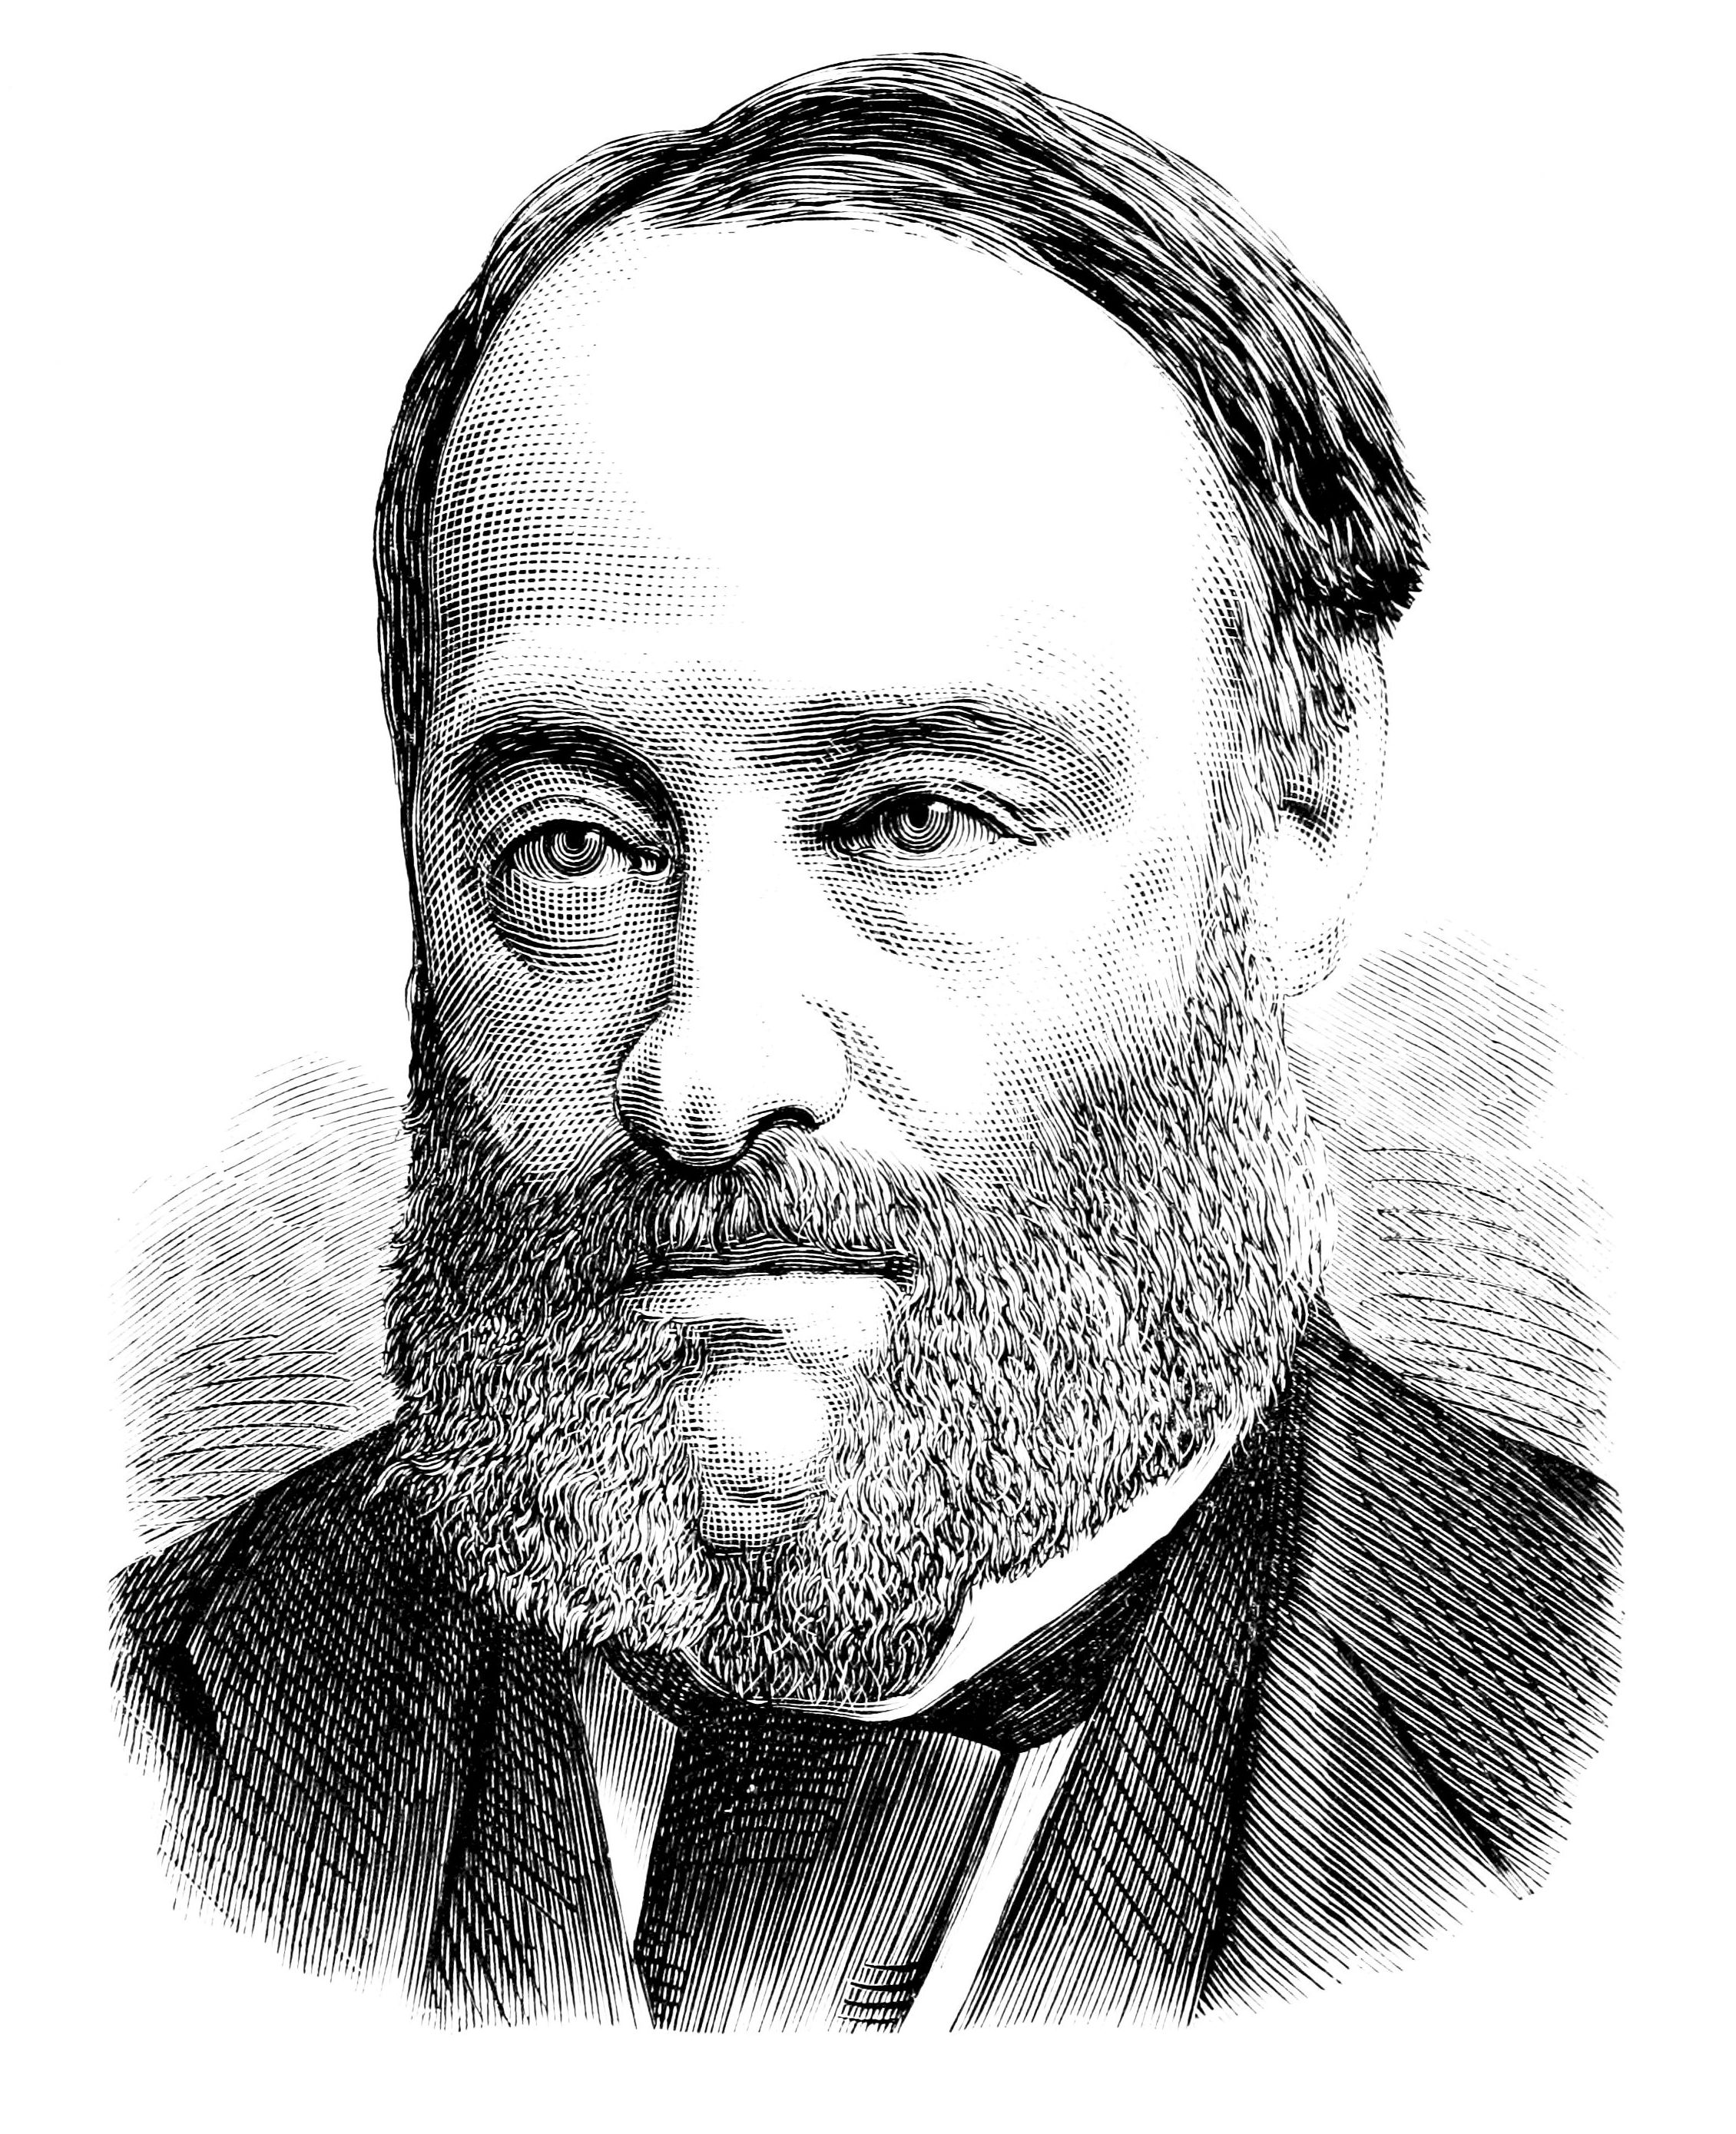
\includegraphics[width=0.92\textwidth]{images/joule.jpg}
\captionof{figure}{James Prescott Joule (1818--1889), portrait by John Collier (1882).}
\end{minipage}\hfill
\begin{minipage}{0.68\textwidth}
In the 1840s, the English physicist and brewer James Prescott Joule conducted meticulous experiments using falling weights to drive paddle wheels immersed in thermally insulated water tanks. 

By measuring the precise mechanical work performed by the descending weights ($\Delta W = mgh$) and the resulting infinitesimal temperature rise of the water, Joule established that mechanical work and thermal energy are interchangeable manifestations of a single universal quantity: \textbf{energy}. His canonical value ($4.18\ \mathrm{J\cdot cal^{-1}}$) shattered the caloric fluid theory and laid the empirical foundation for the First Law of Thermodynamics and the principle of conservation of energy.
\end{minipage}
\end{historicalbox}

\section{Kinetic Energy and the Work-Energy Theorem}

We now establish the mathematical connection between the total work done by all forces and the kinematic state of the particle.

\begin{definitionbox}{Kinetic Energy of a Material Point}
The \textbf{kinetic energy} $E_k$ (also denoted $K$ or $T$) of a point particle of inertial mass $m$ moving at speed $v = \norm{\vec{v}}$ in an inertial reference frame $\mathcal{R}$ is defined as:
\begin{equation}
E_k \eqdef \frac{1}{2} m v^2 = \frac{1}{2} m (\vec{v} \cdot \vec{v}) = \frac{\norm{\vec{p}}^2}{2m}.
\end{equation}
Kinetic energy is an intrinsically positive scalar quantity ($E_k \ge 0$), vanishing if and only if the particle is instantaneously at rest in $\mathcal{R}$.
\end{definitionbox}

\begin{lawbox}{The Work-Energy Theorem (Kinetic Energy Theorem)}
In an inertial frame of reference $\mathcal{R}$, the change in kinetic energy of a material point between any two positions $A$ and $B$ along its trajectory equals the algebraic sum of the work performed by \textbf{all} forces (conservative, non-conservative, internal, and external) acting on the particle:
\begin{equation}
\Delta E_k = E_k(B) - E_k(A) = W_{A \to B}^{\text{net}} = \sum_i W_{A \to B}(\vec{F}_i).
\end{equation}
In differential form, the instantaneous rate of change of kinetic energy equals the net instantaneous power:
\begin{equation}
\frac{\dd E_k}{\dd t} = \mathcal{P}_{\text{net}}(t) = \vec{F}_{\text{net}} \cdot \vec{v}.
\end{equation}
\end{lawbox}

\paragraph{First-Principles Mathematical Proof.}
Let $\vec{F}_{\text{net}} = \sum_i \vec{F}_i$. According to Newton's second law, $\vec{F}_{\text{net}} = m \frac{\dd\vec{v}}{\dd t}$. Differentiating the scalar kinetic energy with respect to time yields:
\[
\frac{\dd E_k}{\dd t} = \frac{\dd}{\dd t}\left(\frac{1}{2} m \vec{v}\cdot\vec{v}\right) = \frac{1}{2}m\left( \frac{\dd\vec{v}}{\dd t}\cdot\vec{v} + \vec{v}\cdot\frac{\dd\vec{v}}{\dd t} \right) = m \vec{v}\cdot\frac{\dd\vec{v}}{\dd t}.
\]
Substituting Newton's law $m\,\dd\vec{v}/\dd t = \vec{F}_{\text{net}}$:
\[
\frac{\dd E_k}{\dd t} = \vec{F}_{\text{net}} \cdot \vec{v} = \mathcal{P}_{\text{net}}(t).
\]
Multiplying by $\dd t$ yields the differential identity $\dd E_k = \vec{F}_{\text{net}}\cdot\dd\vec{r} = \delta W_{\text{net}}$. Integrating both sides along the trajectory from $t_A$ to $t_B$ gives:
\[
\int_{A}^B \dd E_k = E_k(B) - E_k(A) = \int_{A}^B \vec{F}_{\text{net}} \cdot \dd\vec{r} = W_{A \to B}^{\text{net}},
\]
completing the rigorous proof. $\blacksquare$

\subsection{Work-Energy Theorem in Non-Inertial Frames}

In a non-inertial frame of reference $\mathcal{R}'$, Newton's second law includes inertial fictitious forces:
\[
m\vec{a}_r = \vec{F}_{\text{real}} + \vec{F}_{\text{ie}} + \vec{F}_{\text{ic}},
\]
where $\vec{F}_{\text{ie}} = -m\vec{a}_e$ is the entrainment force and $\vec{F}_{\text{ic}} = -2m(\vec{\Omega}\times\vec{v}_r)$ is the Coriolis force.

Projecting onto the relative velocity $\vec{v}_r$:
\[
\frac{\dd E_k'}{\dd t} = m\vec{v}_r \cdot \vec{a}_r = \vec{F}_{\text{real}} \cdot \vec{v}_r + \vec{F}_{\text{ie}} \cdot \vec{v}_r + \vec{F}_{\text{ic}} \cdot \vec{v}_r.
\]
Crucially, the Coriolis force is identically perpendicular to the relative velocity:
\[
\vec{F}_{\text{ic}} \cdot \vec{v}_r = -2m (\vec{\Omega} \times \vec{v}_r) \cdot \vec{v}_r \equiv 0.
\]
\begin{lawbox}{Work of Inertial Forces}
The Coriolis force performs \textbf{strictly zero mechanical work} in all non-inertial frames:
\begin{equation}
\mathcal{P}_{\text{Coriolis}} \equiv 0, \qquad W_{\text{Coriolis}} \equiv 0.
\end{equation}
The Work-Energy theorem in a non-inertial frame $\mathcal{R}'$ reads:
\begin{equation}
\Delta E_k' = W^{\text{real}} + W_{\text{ie}},
\end{equation}
where $W_{\text{ie}} = \int \vec{F}_{\text{ie}}\cdot\dd\vec{r}'$ is the work of entrainment forces (e.g., the centrifugal force).
\end{lawbox}

\begin{cautionbox}[Common Pitfall: The Inexactness of Work]
Never write ``$\Delta W = W_B - W_A$''. Work is \emph{not} a property possessed by a body. A body possesses mass, momentum, and energy, but it \emph{does not} possess work. Work is an energy flux in transit across the system boundary during a process. The notation $W_{A\to B}$ denotes the integrated integral along a specified path.
\end{cautionbox}

\section{Comprehensive Worked Examples}

\begin{workedexample}{The Vertical Loop-the-Loop Roller Coaster}
A small block of mass $m$ slides from rest down a frictionless track that terminates in a circular vertical loop of radius $R$. The block is released from an initial height $h$ above the lowest point of the track $O$. Gravity $\vec{g} = -g\,\khat$ acts vertically downward.
\begin{enumerate}[leftmargin=1.4em,itemsep=3pt]
  \item Determine the speed $v(\theta)$ and the normal reaction force $N(\theta)$ exerted by the track as a function of the polar angle $\theta \in [0, \pi]$ measured from the bottom of the loop.
  \item Find the critical minimum release height $h_{\min}$ required for the block to negotiate the entire loop without losing contact with the track.
  \item Calculate the normal contact force experienced at the lowest point $\theta = 0$ when released from $h = h_{\min}$.
\end{enumerate}

\paragraph{Solution.}
\textbf{1. Speed and Normal Force via Work-Energy Theorem:}\\
Between the release point (height $h$, speed $v_0 = 0$) and an arbitrary position on the loop at angle $\theta$, the height above the bottom is:
\[
z(\theta) = R(1 - \cos\theta).
\]
The forces acting on the block are the weight $\vec{P} = m\vec{g}$ and the track normal reaction $\vec{N} = -N(\theta)\,\ur$ directed inward toward the center. Because the track is frictionless, the normal force is orthogonal to the displacement at every point: $\vec{N}\cdot\dd\vec{r} = 0$, so $W(\vec{N}) = 0$.

The work done by gravity as the particle descends from $z_1 = h$ to $z_2 = z(\theta)$ is:
\[
W(\vec{P}) = -mg\,\Delta z = mg\left(h - R(1 - \cos\theta)\right).
\]
Applying the Work-Energy Theorem $\Delta E_k = W_{\text{net}}$:
\[
\frac{1}{2} m v(\theta)^2 - 0 = mg\left(h - R(1 - \cos\theta)\right) \implies v^2(\theta) = 2g\left(h - R(1 - \cos\theta)\right).
\]
To find the normal contact force $N(\theta)$, we project Newton's second law onto the inward normal unit vector $\un = -\ur$ in the Frenet frame:
\[
\sum F_n = m a_n \implies N(\theta) - mg\cos\theta = m \frac{v^2(\theta)}{R}.
\]
Substituting the expression for $v^2(\theta)$:
\[
N(\theta) = mg\cos\theta + \frac{m}{R}\left[ 2g(h - R + R\cos\theta) \right] = \frac{mg}{R}\left( 2h - 2R + 3R\cos\theta \right).
\]

\textbf{2. Critical Release Height $h_{\min}$:}\\
For the block to remain in continuous contact with the track, the normal reaction must remain non-negative: $N(\theta) \ge 0$ for all $\theta \in [0, \pi]$. Since $\cos\theta$ is monotonically decreasing from $+1$ to $-1$, $N(\theta)$ attains its global minimum at the apex of the loop ($\theta = \pi$, where $\cos\pi = -1$):
\[
N(\pi) = \frac{mg}{R}\left( 2h - 2R - 3R \right) = \frac{mg}{R}(2h - 5R).
\]
The threshold of detachment occurs when $N(\pi) = 0$:
\[
2h_{\min} - 5R = 0 \implies h_{\min} = \frac{5}{2}R = 2.5\,R.
\]
At this critical height, the speed at the summit is $v_{\text{top}} = \sqrt{2g(2.5R - 2R)} = \sqrt{gR}$, exactly balancing centrifugal effect and gravity ($g = v^2/R$).

\textbf{3. Normal Force at the Lowest Point:}\\
Evaluating $N(0)$ with $\theta = 0$ ($\cos 0 = 1$) and $h = \frac{5}{2}R$:
\[
N(0) = \frac{mg}{R}\left( 2\left(\frac{5}{2}R\right) - 2R + 3R \right) = \frac{mg}{R}(5R - 2R + 3R) = 6mg.
\]
The track must exert a normal force equal to \textbf{six times} the body's resting weight at the bottom of the loop to simultaneously support gravity and provide the necessary centripetal acceleration.
\end{workedexample}

\begin{workedexample}{Detachment from a Frictionless Spherical Dome}
A small ice pellet of mass $m$ rests at the apex of a fixed frictionless spherical dome of radius $R$. Given an infinitesimal nudge, it slides down the dome under gravity.
\begin{enumerate}[leftmargin=1.4em,itemsep=3pt]
  \item Derive the speed of the pellet as a function of the polar angle $\theta$ measured from the vertical apex.
  \item Compute the normal contact force $N(\theta)$ exerted by the dome.
  \item Determine the exact polar angle $\theta_{\text{detach}}$, the height $z_{\text{detach}}$, and the velocity at the instant the pellet flies off the surface.
\end{enumerate}

\paragraph{Solution.}
\textbf{1. Speed via Work-Energy Theorem:}\\
Placing the origin at the center of the sphere, the apex is at vertical coordinate $z_0 = R$. At polar angle $\theta$, the vertical height is $z(\theta) = R\cos\theta$.

Since the dome is frictionless, $\vec{N} = N(\theta)\,\ur$ is purely radial and perpendicular to the displacement $\dd\vec{r} = R\,\dd\theta\,\ut$. Thus $W(\vec{N}) = 0$.
The work done by gravity during the descent from $z_0 = R$ to $z(\theta) = R\cos\theta$ is:
\[
W(\vec{P}) = -mg\,\Delta z = mg(R - R\cos\theta) = mgR(1 - \cos\theta).
\]
By the Work-Energy Theorem, assuming an infinitesimal initial speed $v_0 \to 0$:
\[
\frac{1}{2}mv^2 - 0 = mgR(1 - \cos\theta) \implies v(\theta) = \sqrt{2gR(1 - \cos\theta)}.
\]

\textbf{2. Normal Contact Force:}\\
In plane polar coordinates with basis $(\ur, \ut)$, the forces are:
\[
\vec{P} = mg\cos\theta\,\ur - mg\sin\theta\,\ut, \qquad \vec{N} = N(\theta)\,\ur.
\]
The radial equation of motion (projecting along $-\ur$, directed toward the center) is:
\[
\sum F_{\text{inward}} = mg\cos\theta - N(\theta) = m a_n = m \frac{v^2}{R}.
\]
Substituting $v^2 = 2gR(1 - \cos\theta)$:
\[
N(\theta) = mg\cos\theta - \frac{m}{R}\left[ 2gR(1 - \cos\theta) \right] = mg(3\cos\theta - 2).
\]

\textbf{3. Angle, Height, and Speed at Detachment:}\\
The dome cannot pull on the pellet; it can only push ($N(\theta) \ge 0$). Detachment occurs precisely when the contact force vanishes, $N(\theta_{\text{detach}}) = 0$:
\[
3\cos\theta_{\text{detach}} - 2 = 0 \implies \cos\theta_{\text{detach}} = \frac{2}{3}.
\]
The exact detachment angle is:
\[
\theta_{\text{detach}} = \arccos\left(\frac{2}{3}\right) \approx 48.19^\circ \approx 0.8411\ \mathrm{rad}.
\]
The height of detachment above the base of the hemisphere is:
\[
z_{\text{detach}} = R\cos\theta_{\text{detach}} = \frac{2}{3}R.
\]
The pellet has fallen through a vertical drop of $\Delta z = R - \frac{2}{3}R = \frac{1}{3}R$.
Its speed at the instant of detachment is:
\[
v_{\text{detach}} = \sqrt{2gR\left(1 - \frac{2}{3}\right)} = \sqrt{\frac{2}{3}gR}.
\]
For all subsequent motion $\theta > \theta_{\text{detach}}$, the pellet executes a free projectile parabolic trajectory in vacuum.
\end{workedexample}

\begin{workedexample}{Power Requirements and Acceleration with Aerodynamic Drag}
A sports car of mass $m = 1200\ \mathrm{kg}$ accelerates along a straight horizontal track. The internal combustion engine delivers a constant mechanical power $\mathcal{P}_0 = 180\ \mathrm{kW}$ to the drive wheels. The vehicle encounters an aerodynamic drag force modeled by $F_d = \frac{1}{2} C_d A \rho v^2 = \beta v^2$, where the aerodynamic factor is $\beta = 0.45\ \mathrm{kg\cdot m^{-1}}$.
\begin{enumerate}[leftmargin=1.4em,itemsep=3pt]
  \item Determine the terminal maximum speed $v_{\max}$ of the vehicle.
  \item Formulate the differential equation governing speed $v(t)$ using the Work-Energy theorem (power formulation).
  \item Derive an expression for the distance $x$ required to accelerate from an initial speed $v_1 = 10\ \mathrm{m\cdot s^{-1}}$ to $v_2 = 30\ \mathrm{m\cdot s^{-1}}$.
\end{enumerate}

\paragraph{Solution.}
\textbf{1. Maximum Terminal Speed:}\\
At terminal speed $v_{\max}$, the vehicle is no longer accelerating ($\dd v/\dd t = 0$). By the power formulation of the Work-Energy theorem:
\[
\frac{\dd E_k}{\dd t} = \mathcal{P}_{\text{net}} = \mathcal{P}_{\text{engine}} - \mathcal{P}_{\text{drag}} = 0.
\]
The rate of dissipation by aerodynamic drag is $\mathcal{P}_{\text{drag}} = F_d v = \beta v^3$. Equating engine power to drag power:
\[
\mathcal{P}_0 = \beta v_{\max}^3 \implies v_{\max} = \left(\frac{\mathcal{P}_0}{\beta}\right)^{1/3}.
\]
Plugging in numerical values:
\[
v_{\max} = \left( \frac{180 \times 10^3\ \mathrm{W}}{0.45\ \mathrm{kg\cdot m^{-1}}} \right)^{1/3} = (400\,000)^{1/3} \approx 73.68\ \mathrm{m\cdot s^{-1}} \approx 265.2\ \mathrm{km\cdot h^{-1}}.
\]

\textbf{2. Differential Equation of Motion:}\\
The net power is $\mathcal{P}_{\text{net}} = \mathcal{P}_0 - \beta v^3$. Since $E_k = \frac{1}{2}mv^2$, we have $\frac{\dd E_k}{\dd t} = mv\frac{\dd v}{\dd t}$. Therefore:
\[
mv \frac{\dd v}{\dd t} = \mathcal{P}_0 - \beta v^3 \implies \frac{\dd v}{\dd t} = \frac{\mathcal{P}_0 - \beta v^3}{mv}.
\]

\textbf{3. Distance to Accelerate from $v_1$ to $v_2$:}\\
To find distance $x$ as a function of speed, we employ the kinematic chain rule $\frac{\dd v}{\dd t} = v\frac{\dd v}{\dd x}$:
\[
mv^2 \frac{\dd v}{\dd x} = \mathcal{P}_0 - \beta v^3 \implies \dd x = \frac{m v^2\,\dd v}{\mathcal{P}_0 - \beta v^3}.
\]
Notice the remarkable substitution: let $u = \mathcal{P}_0 - \beta v^3$. Then $\dd u = -3\beta v^2\,\dd v$, so $v^2\,\dd v = -\frac{\dd u}{3\beta}$.
Integrating from $x = 0$ ($v = v_1$) to $x$ ($v = v_2$):
\[
x = \int_{v_1}^{v_2} \frac{m v^2\,\dd v}{\mathcal{P}_0 - \beta v^3} = -\frac{m}{3\beta} \int_{u_1}^{u_2} \frac{\dd u}{u} = \frac{m}{3\beta} \ln\left( \frac{\mathcal{P}_0 - \beta v_1^3}{\mathcal{P}_0 - \beta v_2^3} \right).
\]
Substituting the numerical values:
\[
u_1 = 180\,000 - 0.45(10)^3 = 180\,000 - 450 = 179\,550\ \mathrm{W},
\]
\[
u_2 = 180\,000 - 0.45(30)^3 = 180\,000 - 12\,150 = 167\,850\ \mathrm{W}.
\]
The required acceleration distance is:
\[
x = \frac{1200}{3(0.45)} \ln\left(\frac{179\,550}{167\,850}\right) = \frac{1200}{1.35} \ln(1.0697) \approx 888.89 \times 0.06738 \approx 59.9\ \mathrm{m}.
\]
The scalar power formulation resolved in three lines an integration that would have required difficult vector algebra.
\end{workedexample}
